\chapter{Background and Concepts}
The DevOps and serverless cloud computing services are the two main fields that our work related to. In this chapter we will introduce both of them.
\par
Section 2.1 introduces the Agile software development method, which is the basis of DevOps. Section 2.2 shows the definition of continuous integration and continuous delivery, as one of the most important practices of the DevOps. Section 2.3 presents the definition, components of DevOps, also, the definition and components of a DevOps toolchain. Section 2.4 introduces serverless computing, including it's concept, characteristics and limitations.
\section{Agile software development}
\label{agile}
The term "Agile" represents the fast adaptation and response to the changes in the plan \cite{highsmith2002agile}.
Agile software development is a method of software development that implements the ideology of "agile". Agile software development advocates the continuous development of software teams. The software development under this methodology will have shorter planning/development time before it delivers to the customers and could better adapt to changes in the environment and requirements.
\paragraph{Iterative Software Development:} Agile software development uses an iterative way in the development process. The traditional software development process, like the waterfall method, requires the long and complicated planning process, and a complicated document. Once one phase of the development is done, the teams should not change the output (document and code) of this phase \cite{cusumano1995beyond}. In contrast, agile software development aims to satisfy the customer with early and continuous delivery of the software \cite{beck2001manifesto}. "Early" means the shorter time before software delivery. "Continuous" means the development does not end with the delivery. The "delivery" means to an end of an iteration, which comes with a demonstration to stakeholders. After delivery, the team continues to the next iteration according to the feedback it gets from stakeholders. In each iteration, the aim of the team is not to add major features to the software, rather is to have a working and deliverable release \cite{beck1999embracing}. In the ideology of agile, the best design of the software product comes from the iterative development \cite{beck2001manifesto}, rather than the tedious planning. 
\paragraph{High-Quality Software:} The rapid development does not mean low software development quality. On the contrast, the quality of software design is highly appreciated in agile software development. The automated testing is widely used in Agile. The test cases will be defined and implements from the beginning of the development process. The test goes through the entire development iteration to ensure that the software is of high enough quality and can be released or shown to customers at any time during the iteration \cite{Agilesof32:online}.
\paragraph{Collaboration:}
The agile software development processes include collaboration across different groups, i.e. business development team, software development team, test team, and customers. It values face to face communications \cite{beck2001principles} and feedbacks. The purpose of these communications is first to let everyone in the multifunctional agile team understand the whole project, and second to receive feedback that helps the software in the right development track. The track which aligns with the requirement of the stakeholders \cite{beck2001manifesto}. 
\par
According to the Manifesto for Agile Software Development, compared with traditional software development, the agile software development value these aspects \cite{beck2001manifesto}: 
\begin{itemize}
\item Individuals and interactions over processes and tools.
\item Working software over comprehensive documentation.
\item Customer collaboration over contract negotiation.
\item Responding to change over following a plan.
\end{itemize}
\section{Continuous Integration \& Continuous Delivery}
In the software development, CI/CD refers to continuous integration, continuous delivery and continuous deployment \cite{pittet2018continuous}. As we mentioned in \ref{agile}, agile software development requires continuous software quality assurance and iterative development. Currently, CI/CD is one set of the necessary practices for the team to become agile by achieving the requirements above. Figure \ref{fig:cicd} shows the relationship between these 3 practices.
\begin{figure}[h]
    \centering
    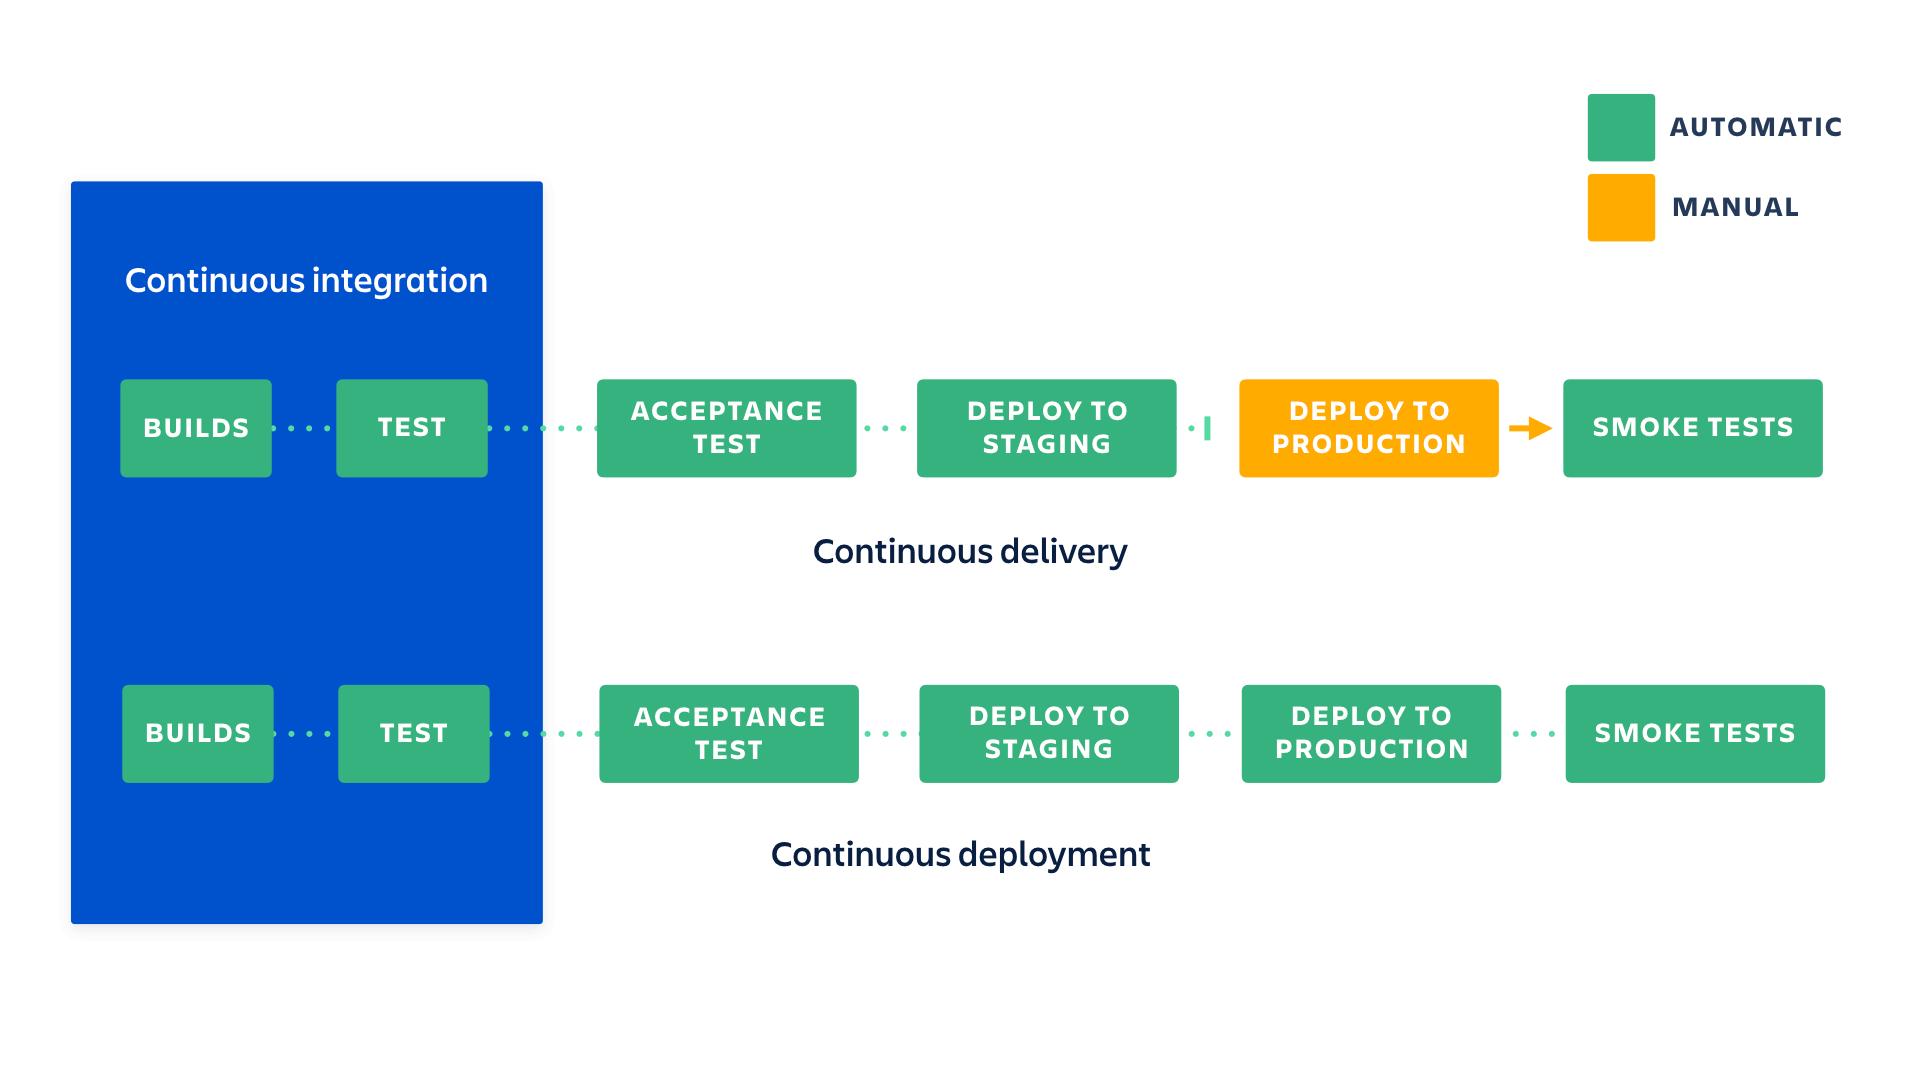
\includegraphics[width=0.95\textwidth]{pics/cicd.png}
    \caption{The relationship between continuous integration, continuous delivery and continuous deployment \cite{pittet2018continuous}}
    \label{fig:cicd}
\end{figure}
\subsection{Continuous Integration}
Continuous integration is the base practice of all practices within CI/CD, and continuous delivery/deployment is based on the continuous integration \cite{pittet2018continuous}.
The continuous integration means the team integrate each team member's work into the main codebase frequently(multiple times per day). "Integrate" means merge the code into the main codebase \cite{fowler2006continuous}. The continuous integration rely on following practices: \textit{Source Code Management}, \textit{Build Automation}, \textit{Visibility} and \textit{Test Automation}. The definition of these practices are:
\begin{itemize}
    \label{TestA}
    \item \textit{Test Automation:} Test automation means using separate software to execute the software automated without human intervention. It could help the team to test fast and test early \cite{Testauto48:online}. There are three approaches to test automation: first, the automated unit tests which design by developers in the early stage of the project. Unit testing aims to verify if each component of the software project works properly; Second, the functional testing which tests the business logic behind the user interface. The function testing is a type of black-box test which the tester only care about if the output is as expected under certain input; Third, the graphical user interface (GUI) testing test if the user interface meets the functionality requirement. The context of GUI testing is to simulate the user's operation on the user interface.
    \item \textit{Build Automation:} Automate the process of creating software build. This means to automate the dependency configuration, source code compiling, packaging and testing. It is viewed as the first step to continuous integration \cite{Buildaut62:online}. There are two types of build automation tools, the build-automation utility and build-automation servers \cite{ceruzzi2003history}. Build-automation utility means the tool to generate build artifacts by compiling the source codes. The common tools that belong to this type include Cmake, Gradle and MSBuild. Build-automation server is the tool which executing build-utility tools; it allows the build to be triggered from the outside or be scheduled on a time basis. Build-automation server is usually web-based. Continuous integration servers, such as Jenkins and Circle CI, is considered as build-automation server. 
    \item \textit{Source Code Management:} In continuous integration, the team, maintains a single source repository and use version control system. In practice, this means one branch in the version control system act as the "mainline", while everyone works off this mainline \cite{fowler2006continuous}. However, everyone needs to merge the code to the mainline every day. For making sure that the mainline code still works after the merge, the mainline that merge the new code needs to be built and tested. we will further introduce this practice in Section \ref{vcs}. 
\end{itemize}
With the help of these practices, the workflow \cite{fowler2006continuous} in continuous integration for each developer in the software team is as follows: In the development of each feature, the developer first pulls the code from the main codebase. During the development, new test cases should also be added to the automated unit test. Automated unit test runs on the code after the developer finishes the feature development. This is for maintaining the code quality and minimise the number of bugs from the beginning. The actual practice for implementing this step is to have build automation tools compiled the code locally in the development machine. 
\par
After the step above, the developer already has the executable and the high quality (passed the automated test) code in the development machine before submitting the change to the repository. This represents the principle of quality and automation in agile software development. In the next step, the developer commits changes to the repository, which is the main codebase, and the system check the conflict and do the test/build again, to make sure that there are not any bugs missed in the test on the development machine.
If the code passes this build and test, it will be merged to the main codebase, and the integration is done.
\subsection{Continuous Delivery and Continuous Deployment}
\label{CD}
Continuous delivery is a practice that the software development team build software that can be released at any time during the life cycle \cite{fowler2013continuous}. This practice ensures that the software always high-quality and in a deployable state \cite{WhatisCo47:online}. Continuous delivery provides a clear way for software development teams to become agile \cite{Whyagile27:online}\cite{IsContin85:online}. In the last section, we introduce the concept of continuous integration.  Continuous delivery is based on continuous integration, but it further automates the software deployment process. In the software deployment pipeline, the team divides the build into several stages, first build the product, and then push the product into a production-like environment for further testing. This ensures that the software can be deployed at any time. However, in continuous delivery, deploying software to the production environment is done manually.
The benefit \cite{WhatisCo47:online}\cite{fowler2013continuous} of continuous delivery includes:
\begin{itemize}
    \item High quality of code: The automate and continuous testing ensure the high quality of code.
    \item Low risk: The software team could release the software at any time. The release process is easy, and it is also harder to make a mistake.
    \item Short time before going to the market: The iteration of software development is much shorter. The automated testing, deployment and environment configuration short the development life cycle. The always ready-to-deploy status shorten the time from development to market.
\end{itemize}
The continuous deployment is based on continuous delivery. The only difference is continuous deployment automates the deployment process. In continuous delivery, the software is deployable but not deployed without manual approval. In the continuous deployment, each change that passed automated build and testing will be deployed directly.
Continuous deployment is a relatively new concept, and most companies have not yet put this practice into production \cite{leppanen2015highways}. Although continuous delivery is a necessary practice for companies to become DevOps, it has been widely used.
\section{DevOps}
\begin{quotation}
    The fundamental goal of DevOps is to minimise the service overhead so that it can respond to change with minimal effort and deliver the maximum amount of value during its lifetime.
    \begin{flushright}
        -- Markus Suonto, Senior DevOps Consultant, Eficode
    \end{flushright}
\end{quotation}
\label{devops}
DevOps is a set of practices that aims to combine different, traditionally separated disciplines (e.g. software development, operations, QA, and others) in cross-functional teams with the help of automation of work to speed up software delivery without risking high-quality \cite{bass2015devops}.
\subsection{Emergence of DevOps}
In the pre-DevOps era, development and operations were two different teams with different goals. The interaction between them is based on the ticket system, and the operation team performs ticket management. As we mentioned at Section \ref{agile}, the goal of Agile is to shorten the deliver life cycle and quickly delivery software to the customers. Therefore, when practising agile development methods in this situation, developers try to deliver code, and they will develop earlier.
However, the operation team usually will delay the process for quality control or other reasons. In practice, this causes the delay between the code change and the software delivery to the customers \cite{leite2019survey}. The lack of communication and conflict between developers and the operation team slow down the software delivery process and also make it harder for the teams to be real Agile. Therefore the concept "DevOps" is being proposed at 2008, for eliminating of the boundary between developers (Dev) and operation team (Ops).
\begin{figure}[h]
    \centering
    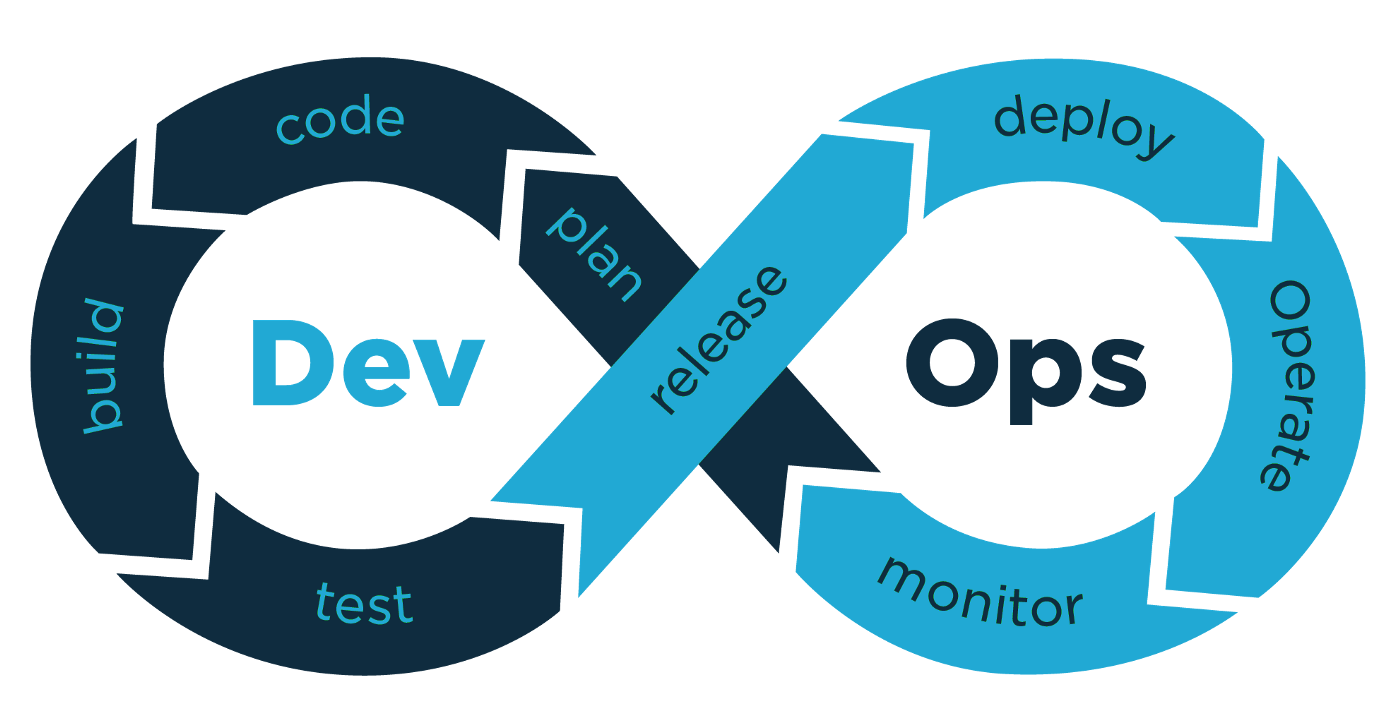
\includegraphics[width=0.95\textwidth]{pics/DevOps.png}
    \caption{DevOps Practices and Workflow \cite{DevOpsin72:online}}
    \label{fig:DevOps}
\end{figure}
\subsection{Relationship with Agile}
DevOps is the extension and evolution \cite{lwakatare2016relationship}\cite{leite2019survey} of Agile. DevOps and Agile both driven by the collaboration ideology and the adoption of DevOps needs Agile as the key factor \cite{lwakatare2016relationship}. DevOps has a different focus on agile. DevOps focus on the whole delivery and customer satisfaction while agile is focused on the development with the requirement and customer \cite{buchanan2015agile}. Figure \ref{fig:DevOps} shows the workflow and practices of a team working under DevOps.
\subsection{Elements}
In this section, we will introduce the necessary elements that an organisation need to includes while introducing DevOps as a common practice.
Eficode proposed it's DevOps capability model which act as the baseline for the DevOps transformation. This model consists following elements enablement, organisation and culture, environments and release, builds and continuous integration,  quality assurance, visibility and reporting, technologies and architecture. Combined with our research that based on other materials related to DevOps, we summarise the DevOps capability model at a more general level, into four aspects.
\subsubsection[]{Culture}
 According to Walls (2013), this is being done by promoting the culture with 4 characteristics open communication, incentive and responsibility alignment, respect and trust \cite{walls2013building}.
\par 
\textbf{Open communication} means open discussion and debate. Communication can help minimise the gap between developers and operations teams. Traditionally, communication within the team is carried out through a very formal and standardised ticketing system.
However, in teams adopting DevOps, communication is not limited to the ticket system. Instead, the team will maintain free communication throughout the life cycle of the product, and they will discuss requirements, timetables, and anything else. In addition, information sharing is also very important\cite{lwakatare2015dimensions}. Metrics and project status are available to everyone in the team \label{moniter}, so each member can clearly understand the scope of the team's work.
\par
The \textbf{incentive and responsibility alignment} mean the entire team (consisting of Dev and Ops) has the same goals and assumes the same responsibilities. The transition from "Dev" and "Ops" to DevOps requires people who used in charges in only development and operation start taking the responsibility in both side \cite{lwakatare2015dimensions}.
Such transition means if the product is failed, individuals or part of the team will be not solely blamed. 
This "no blame" culture could help each engineer be willing to take the development responsibility for the whole system \cite{feitelson2013development}.
\par 
\textbf{Respect} means all employees should respect and recognise the contribution of other teams members. A DevOps team is not a single team without any division of jobs, there is still an operation part within a team \cite{TheresNo86:online}. Therefore each part of the team need to \textbf{trust} the other parts are doing the best to benefit the whole team.
On the other hand, the person in the operation team will take development responsibility, and the developers will also put their hands-on operation and management\cite{shropshire2017uncertainty}. To make people with different roles works in a team, trust and respect each other is critically important. 
\subsubsection[]{Organisation}
In the organisational level, the DevOps emphasises the collaboration between different parts of an organisation. This is closely related to the "culture" part of this section. 
Within a team, each member should be a generalist who could understand all aspects of a project. There will not be a dedicated QA, operation or security team within a team. Instead, these are jobs that belong to everyone \cite{feitelson2013development}\cite{kim2016devops}. The structure and rule of the organisation should provide all members with opportunities to learn all skills needed for building the whole system. 
\par
The DevOps Handbook \cite{kim2016devops} published in 2016, proposed ways to organise an organisation for DevOps transformation. One of the principles in organising the teams is to keep the team boundary and comply with the "two pizza rule" proposed Amazon in 2002. The rule is to keep the team size small for having a more productive team meeting.
A small team could help to reduce the inter-team communication, keep the team scope bounded and small \cite{kim2016devops}. Furthermore, the smaller team also means less bureaucracy in team management. There are four benefits to have a small team:
\begin{itemize}
    \item The smaller team allows each team member to understand the whole project easily.
    \item The smaller team could reduce the amount of communication needed. It could also limit the growth rate that the product could have.
    \item The smaller team could decentralise power. In DevOps, each team lead could define the metrics which become the overall criteria of the whole team's performance.
    \item In a smaller team, failure does not mean a disaster for the company. This fact allows the team to fail. Thus each employee could train their headship skill in the team without too much pressure. 
\end{itemize} 
\par
Having a loosely-coupled architecture is another important organisational aspect for DevOps. The first benefit is the better safety. In the organisation with a tightly-coupled architecture, because each component is closely coped with each other, even a small change could result in large failure \cite{kim2016devops}. The second benefit of the loosely-coupled architecture is productive. In a traditional organisation, the whole organisation shares the same development life cycle. The result of each team will be merged, tested together and deployed together, which is time costly when configuring the test environment and dependencies. A loose organisation enables each team to finish the development life cycle (from planning to deployment) independently. Each team could update their products independently, which gives the team more flexibility to align the product with the change in the customer requirement. 
The update of each team's product should not affect other teams product. 
\subsubsection[]{Automation}
In the DevOps, automation means 
automation within the whole development and operation process. The organisations which employ DevOps aim for a high degree of automation\cite{erich2017qualitative}.
With automation, people could be free from the repetitive work and reduce human error. It could help build the DevOps culture of collaboration, and it is seen as the cornerstone of the DevOps \cite{DevOpsCu76:online}.
The main practices regarding automation are the automated testing, continuous delivery and automated operation. The automation operation includes several practices such as automated monitoring and alarming, automation infrastructure provision and environment configuration.
\par
The continuous delivery pipeline is the core of automation within the scope of DevOps. As per discussed at \ref{CD}, the continuous delivery will ultimately automate all steps between the developer to commit the code to the product in the production. In addition, the continuous pipeline brings together all automated steps within DevOps life cycle.
\par
\label{iasc}
Infrastructure as code is a practice which helps to achieve automated operation part, specificity, environment configuration and infrastructure provision. The Infrastructure as Code (IaC) means everything at the software infrastructure level is defined as code \cite{artac2017devops}. Because it is code, the developer could use the automation methodology used in the software development to manages and deploy these codes. According to Christof et. (2016), under IaC, infrastructure can be shared, tested, and version-controlled \cite{ebert2016devops}. This could help emphasise the automation within the operation scope. In addition, IaC the team could be free from the tedious environment configuration and shorten the product development lifecycle. Automating server configuration with IaC helps the developers and operation staff know the server configuration equally \cite{DevOpsCu76:online}, which help build the culture of shared responsibility and trust.
\subsubsection[]{Monitoring and Measurement}
Monitoring is to continuously collect the matrices from the running system. Monitoring provides the team with good visibility on the whole system. The team could get an update on the system status, and find the problems in the system in time. To conducting the monitoring, the monitoring system needs to do the measurement, which is to collect data properly from the system. The measurement is defined as reducing the uncertainty through observation, which producing quantitative result \cite{hering2015measure}. The organisation should properly use the result (metrics).
\par
In the DevOps way of development, the testing is the key to maintain the quality of the software continuously. However, when the product enters the production, we cannot test the software any more. So, we need monitoring to keep track of the status of the product \cite{huttermann2012devops}. According to State of DevOps report from DORA and Google Cloud, the good monitoring structure and the wisely usage of the data from monitoring for making the business decision could improve the software delivery performance \cite{forsgrenaccelerate}. Thus, monitoring is an important component of DevOps.
\par
With monitoring, the software team could keep tracking the status, and maintain the quality of deployed production. Monitoring enables the management teams to track the KPIs during the production. The monitoring has also enabled the team to collect the data from customers' usage behaviour. This helps the agile development team to improve in the next iteration of the product \cite{lwakatare2015dimensions}.
\par
The development of monitoring should be in parallel with the main product, and the monitoring system can be already be used against the "staging deployment" (see Figure \ref{fig:cicd}) at the early stage of the iteration. By the practice of parallel development, the development team can improve the monitoring system continuously together with the main software system. In addition, the parallel development helps the team to find the gap in the monitoring earlier \cite{huttermann2012devops}.
\par
As we mentioned in the "Culture" section, the collaboration is an important part of the DevOps culture. Collaboration needs the communication and information sharing between the development(Dev) and operation(Ops) team. The monitoring could be one of the channels between the Dev and Ops since it can expose the information of the whole system, which helps team members to understand the system as a whole. This helps the team achieving the point we mentioned at \ref{moniter} (Culture) that the project status and matrices should be available to every team members.
\subsection{Toolchain}
A DevOps toolchain is a set of tools that are integrated to aid the software development, deployment and management through the whole software development lifecycle. The goal of DevOps toolchain is to help the software development fits the DevOps principles \cite{DevOpsto7:online}\cite{Toolchai10:online}\cite{WhatisaD20:online}. Within DevOps toolchain, each tool in the toolchain related to a specific activity in DevOps, for example, Jenkins works as automating tasks.
\par
According to \cite{WhatisaD20:online}, DORA state of DevOps reports \cite{forsgrenaccelerate}\cite{velasquez2014state}\cite{forsgren20192019} and our previous definition of the DevOps, we summarise the essential component of a DevOps toolchain as below.
\subsubsection{Project Management \& Planning}
Planning software development project, track the tickets and the issues, communication between and within the teams. The project management tools help to implement the DevOps culture, which enhances collaboration and knowledge sharing.
\subsubsection{Configuration Management}
Configuration management provides a central platform to manage the configuration across the assets. Such a tool allows the team defines the desired state of the assets in a configure file. Then the tool automates the configuration process, which reaching the assets to the defined status. In the cloud environment, a common practice of configuration management is through infrastructure as code, which is define the cloud infrastructure, services configuration and deployment orchestration as configuration file \cite{7965401}.
\subsubsection{Continuous Integration}
Continuous integration (in short: CI) is the top practice for improving the Deployment Frequency \cite{velasquez2014state}. It is one of the most important parts of DevOps toolchain. As we introduced at \ref{CD}, CI allows the developers to integrate their work more frequently to the production products, and it shortens the time to the market of the product. The automatic testing and code analysis integrated into the CI continuously maintain the quality of the product. CI tools also automated the most parts of the software development pipeline, In conclusion, CI helps the system fulfil the DevOps definition (\ref{devops}) by speed up the delivery by automation, maintain the quality by continuous quality assurance. 
The location of the CI server is flexible, depends on the scenario, it could be either on-premises (on a development machine or a local server) or deployed on the cloud. Nowadays, some vendors provide CI as a service. In this case, the CI server is hosted, managed by the vendor and be provided to the user as an online service. As we introduced in \ref{CD}, CI brings together all automation tools, and automate the DevOps workflow, which connects multiple automated processes. CI is the "confluence point" of the most DevOps tools, and thus the core of the whole DevOps toolchain.
\subsubsection{Version Control}
Version control is an important part of DevOps toolchain. It is a system that could record and track the changes in a set of files over time. Version control simplifies the collaboration between team members. Furthermore, allow the simultaneous development of the different parts of a software system. According to \cite{Sourcean53:online} and \cite{velasquez2014state}, version control is the top practice when it comes to improving the multiple metrics in DevOps. Version control becomes the indicator of the software system performance \cite{Sourcean53:online} infrastructure as code. An important DevOps practise we mentioned at \ref{iasc} also relies on version control.
\par
The version control is composed of a repository and the checkout. The repository is a database which records all history versions of the files. The checkout is the local copy of all the files. The user could edit the files in the checkout, then commit the change to the repository. Depends on the location of the repository, there are three types of version control systems \cite{VCS}.
\begin{itemize}
    \item \textbf{Local Version Control Systems:} The repository located locally on the development machine where the user keeps the checkout. However, the repository is stored in a separated version database that keeps all changes of files. 
    \item \textbf{Centralized Version Control Systems:} The repository located in a centralised server, while there are multiple checkouts on multiple development machines. This allows multiple developers to work together under a version control system. However, such setup is not fault-tolerated because to the VCS server is centralised.
    \item \textbf{Distributed Version Control Systems:} This is a type of VCS system that leverage the peer-to-peer approach. Most modern VSC system, such as Git, is using such approaches. The file history is not only kept in the server, but also in each development machine where has the checkout. Once the server dies, the history record will not be lost, and the development machine that retains the file history record will copy the file back after the server is up and running again.
\end{itemize}
\subsubsection{Monitoring}
The monitoring system is one of 4 basic elements of DevOps, as we mentioned at \ref{moniter}. In the DevOps toolchain, the monitoring system detects the failure in the whole system and helps the software team find the problems earlier. The team could also collect performance-related matrices with the help of the monitoring system, which could be used for optimising the application. Besides, the monitoring system can also help in the business aspect by collect the KPI-related metrics form the user's behaviour. Monitoring system combines the data measured from the system and then visualises these data on the dashboard. The visualisation helps people which is not in the operation team understand the data.
\subsubsection{Test Automation}
The test automation tool could verify the code before it being built. Such tools usually come either an independent tool or a plugin that embedded within IDE, build server and continuous delivery pipeline. The integration of testing with other tools such as continuous integration pipeline makes it easy for the organisation to implement the quality gate in the software development \cite{huttermann2012devops}.
The test automation tool runs on the local development machines after each build, after committing to the repository, and before the deployment to production. This policy makes sure that the testing and quality control goes through the whole software life cycle. We will introduce when runs automation testing and what kind of testing will bu run in section \ref{workflow}. 
\section{Serverless Computing}
In this section, we focus on the concepts of Serverless Computing. We will have more discussion regarding the new cloud service based on Serverless Computing in the next chapter.
\par
Serverless Computing (in short: Serverless) is a cloud execution model in which the cloud provider manages the server and resources allocation. 
The popularity of serverless is precipitated by the development of microservices and container technologies \cite{baldini2017serverless}. A survey by the Cloud Native Computing Foundation (CNCF) showed that in 2019, 41\% of respondents used serverless technology in production, compared with 32\% in 2018\cite{cncf2020}. The report of this survey also shows that serverless architectures and cloud functions are being used by 3.3 million developers \cite{cncf2020} in 2019.
\par
In traditional cloud computing services, users rent a fixed number of cloud servers from the cloud provider, and then the cloud provider charges users based on the lease period and server type (pay-as-you-go model). In serverless computing services, developers only pay based on the execution time of the program.
Another difference between serverless computing and traditional computing method is that, in serverless computing, users doesn't need to care about the physical machine that runs the application. In addition, in serverless, the environment that runs the application will be destroyed shortly after the application terminates. 
However, the task is still running on a physical cloud server that is fully managed by the cloud provider. This means that when serverless is used, the user leaves all server provisioning and management tasks to the cloud provider \cite{jonas2019cloud}.
\subsection{History}
In the early days of cloud computing, the consideration behind cloud computing design was that developers only needed to transfer their deployment environment from a local server to a server on the cloud. Therefore, cloud virtual machines (for example, Amazon Web Service EC2) is the main form of providing cloud services.
After Amazon Web Service started offering the service with the virtual machine, Google entered this field for competing with AWS, but in another direction.
In 2008, Google released Google App Engine (GAE) \footnote{https://cloud.google.com/appengine}\cite{zahariev2009google}. The platform allows developers to run their code without managing the cloud virtual machine. This makes Google the first in the main cloud providers to allow the developer to run code on its cloud without provisioning and to manage the cloud servers. However, the GAE only allows the developer to run the python code that is programmed with Google's framework, rather than running arbitrary Python code. 
Amazon Web Service (AWS) introduces AWS Lambda in 2014, make Amazon the first public cloud provider that provides serverless computing platform\cite{Serverle77:online}. Since then the serverless computing starts its rapid commercial development. Following AWS, other providers also introduced their serverless computing platforms. Only in a single year (2016), Google \footnote{https://cloud.google.com/functions}, Microsoft \footnote{https://azure.microsoft.com/en-us/overview/serverless-computing/}, and IBM \footnote{https://www.ibm.com/cloud/functions} released their serverless computing platform respectively. 
In the beginning, the serverless computing offering of vendors is limited to function as a service (FaaS), and the company only use the serverless computing in some supportive components like scheduled tasks.
Nowadays, the serverless is expending it's application scope together with the extension of serverless offering in cloud vendors. For example, AWS provides a serverless platform \footnote{https://aws.amazon.com/serverless/} with the different component for a modern application, as well as tools and services for DevOps. These components are enough for a software team builds microservices architecture backend service for web applications, with DevOps toolchain that also builds in AWS. In a word, the serverless cloud service cloud now covers the entire development life cycle.\label{servlessApp}
\subsection{Characteristics}
We conducted research related to the main characteristics of serverless computing, and we summarise our finding in following four main characteristics based on materials \cite{castro2019rise}\cite{lee2018evaluation}\cite{jonas2019cloud} we read.
\subsubsection{Event Driven}
Event-Driven means the serverless applications is usually triggered and start running due to an event. There are different kinds of event that could act as a trigger. The first one is the HTTP request. When an HTTP request reaches the server, the serverless application could be triggered to reads the context of this request, execute the code, return the HTTP response to the frontend. This kind of pattern matched the nature of web application which allows the developer easily build serverless API for web/mobile applications on top of serverless cloud functions. The serverless application could also be triggered by changes in the database and object storage. This allows the serverless computing to be used as a background task such as data processing. A good example is the serverless computing use case of Thomson Reuters in their social media data analysis project\cite{ThomsonR38:online}. Thomson Reuters uses AWS Lambda to host a serverless application that triggers when new data is stored. The application processes the data real-time, extracts the hashtag trend data and stores it in Amazon DynamoDB, a database solution by AWS, which is also serverless.
\subsubsection{Managed Resources Allocation}
Managed resources allocation means that developers only need to deploy code without leaving operational tasks to the cloud. As we mentioned before The developer does not need provisioning or managing any server besides, the developer is not required to install any software or runtime \cite{Serverle64:online} when deploying his/her application. 
\par
The cloud provider manages the scaling of the infrastructure which the developers are running their code. This also reflects the managed resource allocation of serverless. In traditional virtual machines, although some cloud providers (such as AWS and Azure) support automatic scaling; however, the scaling strategy must be defined by the user. Moreover, the user needs to set up the cloud infrastructure (such as Auto Scaling Groups and Elastic Load Balancing in AWS) for using autoscaling. In contrast, in serverless computing, the cloud provider will handle everything related to automatic scaling.
Furthermore, together with other operational tasks, the availability and security issues of the underlying infrastructure are being taken care of by the cloud provider as well. 
\subsubsection{Pay-per-use}
Pay-per-use is the significant characteristic of serverless computing form non-technical perspective. The traditional cloud server using pay-as-you-go mode. The billing is done based on the type of VM and the rental time of this VM. For the user, this is not economically flexible, because the user must pay the same price for an idle VM as when it is fully loaded. On the contrast, in serverless computing, the users do not need to pay the idle time; they only pay for the time that the application is running. In many scenarios, such payment mode could lower the cost. According to \cite{jonas2019cloud}, serverless computing could be 6x cheaper than VM when doing on-fly video encoding, with 60x performance. An organisation could save up to 4x-10x when moves application to serverless \cite{jonas2019cloud}\cite{Serverle67:online}.
\subsubsection{Extensive Application Scenarios}
Serverless computing has a wide range of applications. A common application is to deploy the runtime in a serverless environment.
However, as mentioned in section \ref{servlessApp}, serverless computing is now not limited to deploy cloud functions but used in all the components that could be used when building modern applications. 
For example, besides serverless functions (AWS Lambda), the serverless offering in AWS also includes the serverless database, container runtime services, data analysis and Kubernetes cluster. Google cloud also advocates "full-stack serverless" \cite{Serverle29:online}. Like AWS, Google Cloud also provides various serverless solutions ranging from computing and DevOps storage to AI and data analysis. Azure's serverless products also cover a wide range of backend components, including computing, storage, artificial intelligence, monitoring and analysis \cite{AzureSer56:online}.
\subsection{Limitations}
\label{servlesslimitation}
Serverless computing is not the perfect solution. In some aspects, it still has it is limitations.
\subsubsection{Performance}
\label{servlesslimitationPer}
This is mainly the problem within the computing task that runs serverless. In the current serverless products of cloud providers, the computing power of serverless computing is limited. 
For example, in the virtual machine service (AWS EC2) provided by AWS, users can choose virtual machines with up to 96 CPUs and 192 GB RAM. In the serverless AWS computing engine, the maximum RAM size allocated is only 3008MB \cite{AWSLambd13:online}, and the maximum number of vCPUs is not specified in the document.
This limits the application scenarios of serverless computing to the development team by making serverless computing services unsuitable for heavy tasks.
In some cases (such as machine learning model training), the limitations of hardware selection are also mimicking performance. Research experiments \cite{jonas2019cloud} at the University of California, Berkeley show that because AWS Lambda does not support GPU computing, makes it 21 times slower than EC2 instances using GPU \cite{hellerstein2018serverless} when training deep learning models. In this case, longer execution times could make serverless servers more expensive, and the research also shows serverless has poor performance in MapReduce and linear
algebra computing. In conclusion, as a development team, selecting serverless computing means limited hardware option and poor performance with a high cost in some scenarios.
\subsubsection{Cold Start}
The cold start is also a disadvantage of serverless. In when running a function on serverless cloud service, the functions are being served by container \cite{KeepingF68:online}. As long as the functions keep bring triggered, the container which hosting the functions will stay active. The cold start means the trigger event happens when the function is not being triggered for a too long time, so the cloud provider has already deactivated the container. In such a situation, the cloud has to deploy the code again and spin up a new container. This will significantly add overhead to the total execution time. 
Thus, if the development team needs to run a short task frequently, but not so frequently to keep the cloud function "warm", serverless is not the best option. This is because the cold start time could take even longer than the actual runtime, which will lower the performance. 
\par
Fortunately, for AWS Lambda, some plugins exist to solve this problem. The common practices of these plugins are to use CloudWatch to ping the function periodically. However, for other serverless services (such as AWS Fargate), there is no way to significantly shorten the cold start time.
\subsubsection{Communication Pattern}
The communication pattern between serverless services is limited: 
In current serverless computing offering from cloud providers, there is a lack of peer-to-peer networking between different running serverless instances \cite{hellerstein2018serverless}. This means some heavy lifting inter-communication such as streaming content to another function \cite{ServerlessNetworking} cannot be done efficiently. For example, in AWS Lambda, replacement of peer-to-peer networking between executing cloud functions is through slow cloud storage \cite{hellerstein2018serverless}. While the communication between virtual machines is through the network interface, which is much faster than cloud storage. Such limitation could further affect the performance of the distributed system that hosted by serverless since the distribute algorithm largely depends on the communication between nodes.
\par
Another limitation is the communication pattern of serverless leads to more inter-instances communication. A good example is the MapReduce \cite{jonas2019cloud}. While in VM part of shuffle and aggregation operation could be done within a VM instance, but between different tasks, such operations in Lambda must require inter-instance communication, since each task is on an independent instance. This problem largely increases the need for network communication. The experiments from UC Berkeley shows that during MapReduce operation, the serverless functions cost 15\% more than VM \cite{jonas2019cloud}.